
\documentclass[conference]{IEEEtran}
\IEEEoverridecommandlockouts

% Configuración para español
\usepackage[spanish,es-nodecimaldot,es-noshorthands]{babel}
\usepackage[utf8]{inputenc}
\usepackage[T1]{fontenc}

% Paquetes IEEE
\usepackage{cite}
\usepackage{amsmath,amssymb,amsfonts}
\usepackage{algorithmic}
\usepackage{graphicx}
\usepackage{textcomp}
\usepackage{xcolor}
\usepackage{float}
\usepackage{listings}
\usepackage{array}
\usepackage{url}

% Configuración de código
\definecolor{codegray}{rgb}{0.45,0.45,0.45}
\definecolor{codeblue}{rgb}{0.10,0.10,0.60}

\lstset{
    basicstyle=\ttfamily\scriptsize,
    keywordstyle=\color{codeblue}\bfseries,
    commentstyle=\color{codegray}\itshape,
    stringstyle=\color{codegray},
    numbers=left,
    numberstyle=\tiny\color{codegray},
    numbersep=5pt,
    frame=single,
    breaklines=true,
    breakatwhitespace=true,
    showstringspaces=false,
    tabsize=2,
    captionpos=b
}

\begin{document}

\title{Práctica 8: Centinela -- Aplicación Completa de un Sistema Embebido}

\author{
    \IEEEauthorblockN{Belmont Muñoz Samuel}
    \IEEEauthorblockA{\textit{Ingeniería en Computación}\\
        \textit{Facultad de Ingeniería}\\
        No. Cuenta: 317318289}
    \and
    \IEEEauthorblockN{Domínguez Palacios Jesús Alejandro}
    \IEEEauthorblockA{\textit{Ingeniería en Computación}\\
        \textit{Facultad de Ingeniería}\\
        No. Cuenta: 421066205}
    \and
    \IEEEauthorblockN{Dorantes Mejía Emmanuel}
    \IEEEauthorblockA{\textit{Ingeniería en Computación}\\
        \textit{Facultad de Ingeniería}\\
        No. Cuenta: 313004766}
    \and
    \IEEEauthorblockN{García Olvera Emiliano}
    \IEEEauthorblockA{\textit{Ingeniería en Computación}\\
        \textit{Facultad de Ingeniería}\\
        No. Cuenta: 314256009}
    \and
    \IEEEauthorblockN{Hernández Alonso Antonio Adonahí}
    \IEEEauthorblockA{\textit{Ingeniería en Computación}\\
        \textit{Facultad de Ingeniería}\\
        No. Cuenta: 320257780}
    \and
    \IEEEauthorblockN{Jiménez Reyes Alan Yael}
    \IEEEauthorblockA{\textit{Ingeniería en Computación}\\
        \textit{Facultad de Ingeniería}\\
        No. Cuenta: 320026726}
}

\maketitle

\begin{center}
    \vspace{-0.3cm}
    {\small
        \textbf{Práctica No.:} 8 \quad | \quad
        \textbf{Grupo:} 6 \quad | \quad
        \textbf{Fecha:} 19/10/2026
    }
    \vspace{0.2cm}
\end{center}

% =====================================================
% RESUMEN
% =====================================================

\begin{abstract}
Este reporte documenta el desarrollo y las pruebas de Centinela, una aplicación de alarma térmica implementada en una Raspberry Pi 4 mediante lenguaje C. El sistema integra un sensor BMP280 para medir temperatura, un potenciómetro conectado mediante el convertidor MCP3008 para establecer un umbral, cuatro LEDs para indicar el estado de vigilancia y dos botones para controlar y consultar el funcionamiento. Se implementó una máquina de estados con las condiciones VIGILANDO, ALARMA y PAUSADO, además de un mecanismo de histéresis para evitar cambios continuos de estado. La práctica incluyó pruebas automáticas de lógica, ejecución sobre hardware real, registro de mediciones en un archivo CSV y evaluación del consumo de CPU con diferentes periodos de muestreo. Se alcanzaron 43 de 43 pruebas de lógica y se analizaron los resultados experimentales, incluyendo los problemas de comunicación observados durante la ejecución y las diferencias entre las configuraciones de eficiencia.
\end{abstract}

\begin{IEEEkeywords}
Sistemas embebidos, Raspberry Pi, Centinela, BMP280, MCP3008, GPIO, máquina de estados, histéresis, CPU, lenguaje C.
\end{IEEEkeywords}

% =====================================================
% OBJETIVOS
% =====================================================

\section{Objetivo}

\subsection{Objetivo General}

Desarrollar e implementar una aplicación de alarma térmica en una Raspberry Pi 4, integrando sensores, actuadores, manejo de archivos y control de estados, para evaluar su funcionamiento y eficiencia mediante pruebas automáticas y experimentales.

\subsection{Objetivos Específicos}

\begin{itemize}
    \item Integrar el sensor BMP280, el convertidor MCP3008, los botones y los LEDs en una aplicación desarrollada en C.
    \item Implementar las funciones de cálculo de temperatura base, umbral, barra de LEDs y transición de estados.
    \item Validar el funcionamiento de las funciones mediante las 43 pruebas automáticas proporcionadas.
    \item Comprobar el comportamiento del sistema en los estados VIGILANDO, ALARMA y PAUSADO.
    \item Registrar las mediciones y los cambios de estado en un archivo CSV.
    \item Evaluar el tiempo de CPU utilizado por el programa con diferentes periodos de muestreo.
    \item Analizar la relación entre frecuencia de lectura, respuesta del sistema y consumo de recursos.
\end{itemize}

% =====================================================
% INTRODUCCIÓN
% =====================================================

\section{Introducción}

Los sistemas embebidos se utilizan para realizar tareas específicas mediante la interacción entre componentes de hardware y software. En aplicaciones de monitoreo, estos sistemas deben adquirir información del entorno, procesarla y ejecutar acciones dependiendo de las condiciones detectadas. Para conseguirlo, es necesario integrar sensores, actuadores, mecanismos de control y herramientas de registro.

En esta práctica se desarrolló Centinela, una alarma térmica implementada en una Raspberry Pi 4. Su funcionamiento consiste en medir la temperatura del ambiente mediante un sensor BMP280 y compararla con un umbral ajustable a través de un potenciómetro. Dependiendo de la diferencia entre ambos valores, el programa controla una barra de cuatro LEDs o activa un patrón de alarma.

La aplicación también incorpora dos botones que permiten pausar el sistema y consultar su estado actual. Asimismo, almacena información de temperatura, umbral y estado en un archivo CSV, permitiendo conservar un historial del funcionamiento.

Uno de los aspectos principales de la práctica fue implementar la lógica mediante una máquina de estados finitos, utilizando histéresis para evitar transiciones repetitivas cuando la temperatura se encuentra cerca del umbral. Además, se evaluó el tiempo de CPU utilizado por la aplicación para identificar configuraciones que permitieran reducir el consumo de recursos sin afectar las funciones principales.

\subsection{Máquina de Estados Finitos}

Una máquina de estados finitos es un modelo de funcionamiento en el que un sistema puede encontrarse en un número determinado de estados. El cambio entre ellos depende de condiciones previamente establecidas.

En Centinela se utilizaron tres estados:

\begin{itemize}
    \item \textbf{VIGILANDO:} El sistema mide la temperatura y representa mediante los LEDs qué tan cerca se encuentra del umbral.
    \item \textbf{ALARMA:} Se activa cuando la temperatura alcanza o supera el umbral. Los LEDs alternan entre dos pares cada 250 ms.
    \item \textbf{PAUSADO:} Desactiva la alarma y apaga los LEDs hasta que el usuario reanuda el sistema.
\end{itemize}

Las transiciones dependen de la temperatura medida, el umbral configurado y la interacción con el botón de pausa.

\subsection{Temperatura Base y Umbral}

Durante el arranque, Centinela calcula una temperatura base a partir del promedio de ocho lecturas del BMP280. Este valor funciona como referencia para establecer el umbral de alarma.

El umbral se calcula mediante:

\begin{equation}
U = T_b + 50 + \frac{P(300)}{1023}
\end{equation}

donde $T_b$ representa la temperatura base en centésimas de grado Celsius y $P$ es la lectura del potenciómetro, comprendida entre 0 y 1023.

De esta manera, el umbral puede ajustarse entre 0.50 y 3.50 grados Celsius por encima de la temperatura base.

\subsection{Histéresis}

La histéresis permite establecer condiciones diferentes para activar y desactivar una alarma. Su finalidad es evitar que pequeñas variaciones en la medición provoquen cambios continuos entre estados.

En Centinela, la alarma se activa cuando:

\begin{equation}
T \geq U
\end{equation}

Mientras que regresa al estado VIGILANDO cuando:

\begin{equation}
T \leq U - 0.30\,^{\circ}\mathrm{C}
\end{equation}

Esto proporciona un margen de estabilidad ante fluctuaciones de temperatura.

\subsection{Registro de Datos y Sincronización}

El sistema utiliza el archivo \texttt{centinela.csv} para almacenar las mediciones realizadas durante su funcionamiento.

Cada registro contiene el tiempo transcurrido en milisegundos, la temperatura, el umbral y el estado actual.

La función \texttt{fsync()} permite solicitar la sincronización de los datos pendientes con el almacenamiento, principalmente durante cambios de estado y al finalizar el programa.

\subsection{Eficiencia del Procesador}

El tiempo de CPU representa el tiempo durante el cual el procesador ejecuta instrucciones de un programa. Este valor puede utilizarse como indicador de la carga computacional.

En Centinela, los periodos de lectura de botones y sensores influyen en la frecuencia con la que se realizan operaciones. Por esta razón, modificar dichos periodos permite estudiar el equilibrio entre capacidad de respuesta y consumo de recursos.

% =====================================================
% DESARROLLO
% =====================================================

\section{Desarrollo}

\subsection{Material y Equipo}

Para la realización de la práctica se utilizaron los siguientes elementos:

\begin{itemize}
    \item Raspberry Pi 4 con Raspberry Pi OS.
    \item Sensor de temperatura y presión BMP280.
    \item Convertidor analógico-digital MCP3008.
    \item Potenciómetro conectado al MCP3008.
    \item Cuatro LEDs conectados a GPIO17, GPIO27, GPIO22 y GPIO23.
    \item Dos botones conectados a GPIO5 y GPIO6.
    \item Protoboard y conexiones de las prácticas anteriores.
    \item Compilador GCC y herramienta Make.
    \item Repositorio Git del equipo.
    \item Kit de archivos \texttt{FSE\_P08\_kit.zip}.
\end{itemize}

El circuito utilizado fue el desarrollado durante las prácticas 2 y 3, manteniendo sus conexiones originales.

\subsection{Organización del Trabajo}

El desarrollo se dividió de acuerdo con las actividades establecidas en la guía de laboratorio. Estas comprendieron la preparación del entorno, implementación de funciones, integración con el circuito, validación del funcionamiento y medición de eficiencia.

Las responsabilidades se distribuyeron entre la integración del programa, desarrollo de las funciones de cálculo, implementación de la máquina de estados, pruebas sobre el circuito y análisis del consumo de CPU.

\subsection{Parte A. Preparación del Kit y Verificación Inicial}

Para comenzar, se descomprimió el archivo \texttt{FSE\_P08\_kit.zip} dentro del directorio de trabajo del equipo. Posteriormente, se ingresó a la carpeta \texttt{p08} y se ejecutó el comando \texttt{make prueba} para conocer el estado inicial del programa.

La primera ejecución reportó únicamente 7 de 43 pruebas superadas. Este resultado era esperado, debido a que las funciones proporcionadas en el kit todavía no contaban con su implementación completa.

En la Figura~\ref{fig:c1} se observa la extracción de los archivos del proyecto y el resultado inicial de las pruebas automáticas.

\begin{figure}[H]
    \centering
    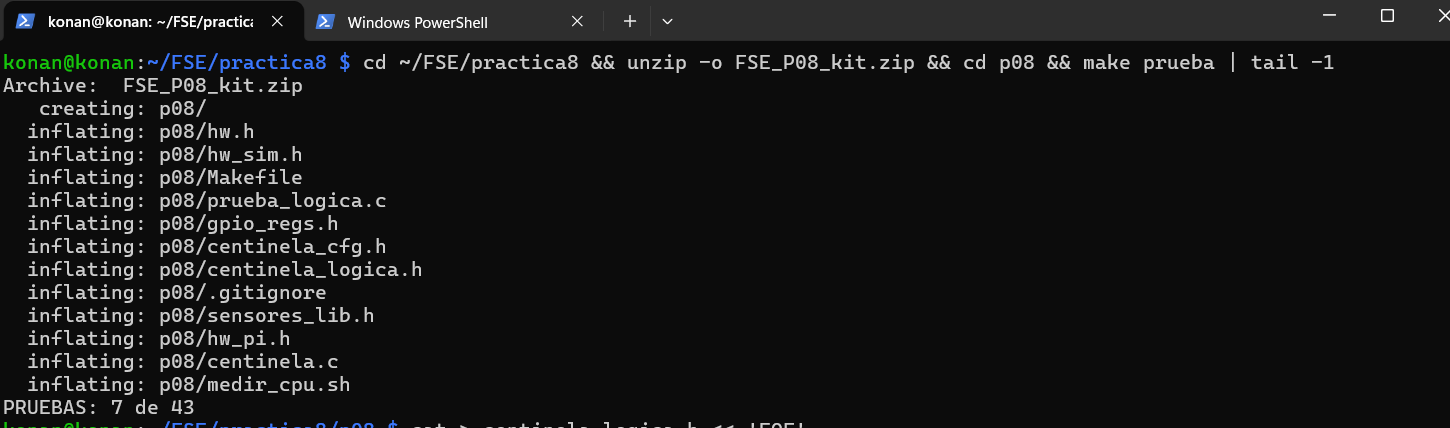
\includegraphics[width=\columnwidth]{C1.png}
    \caption{Descompresión del kit de la práctica y ejecución inicial de las pruebas automáticas, con un resultado de 7 de 43.}
    \label{fig:c1}
\end{figure}

Esta primera evaluación permitió identificar el punto de partida del desarrollo y comprobar que las herramientas de compilación y prueba se encontraban disponibles.

\subsection{Parte B. Implementación de la Lógica}

La segunda etapa consistió en completar las siete funciones definidas en el archivo \texttt{centinela\_logica.h}.

Estas funciones permiten calcular la temperatura base, obtener el umbral mediante el potenciómetro, determinar la cantidad de LEDs encendidos, construir máscaras de bits, generar el patrón de alarma, controlar las transiciones de estado y formatear los registros del archivo CSV.

Para el cálculo de la temperatura base se utilizó un acumulador de 64 bits, con la finalidad de evitar desbordamientos al sumar las lecturas.

En el cálculo del umbral se utilizaron operaciones enteras y conversiones explícitas de tipo para mantener la precisión requerida por las pruebas.

La función de transición de estados consideró las condiciones de pausa, activación de alarma y desactivación mediante histéresis.

Una vez integradas las funciones, se ejecutaron nuevamente las pruebas automáticas.

\begin{figure}[H]
    \centering
    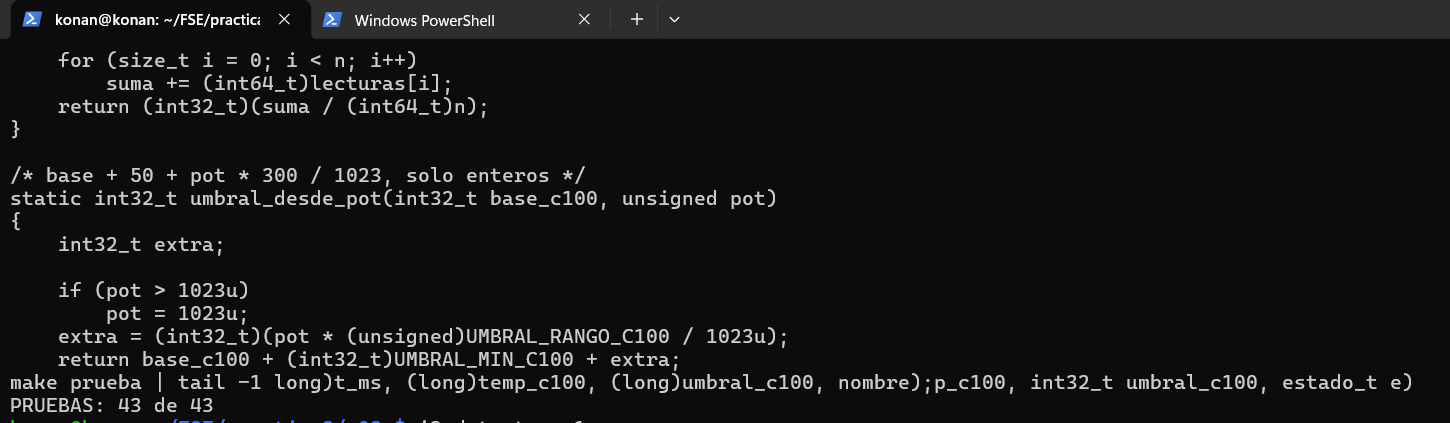
\includegraphics[width=\columnwidth]{C2.png}
    \caption{Implementación de las funciones de cálculo y validación final de la lógica, alcanzando 43 de 43 pruebas.}
    \label{fig:c2}
\end{figure}

Como se muestra en la Figura~\ref{fig:c2}, el programa consiguió superar las 43 pruebas disponibles, comprobando el funcionamiento esperado de la lógica implementada.

Posteriormente, se consultó la plataforma de la liga para verificar el registro de los resultados del equipo.

\begin{figure}[H]
    \centering
    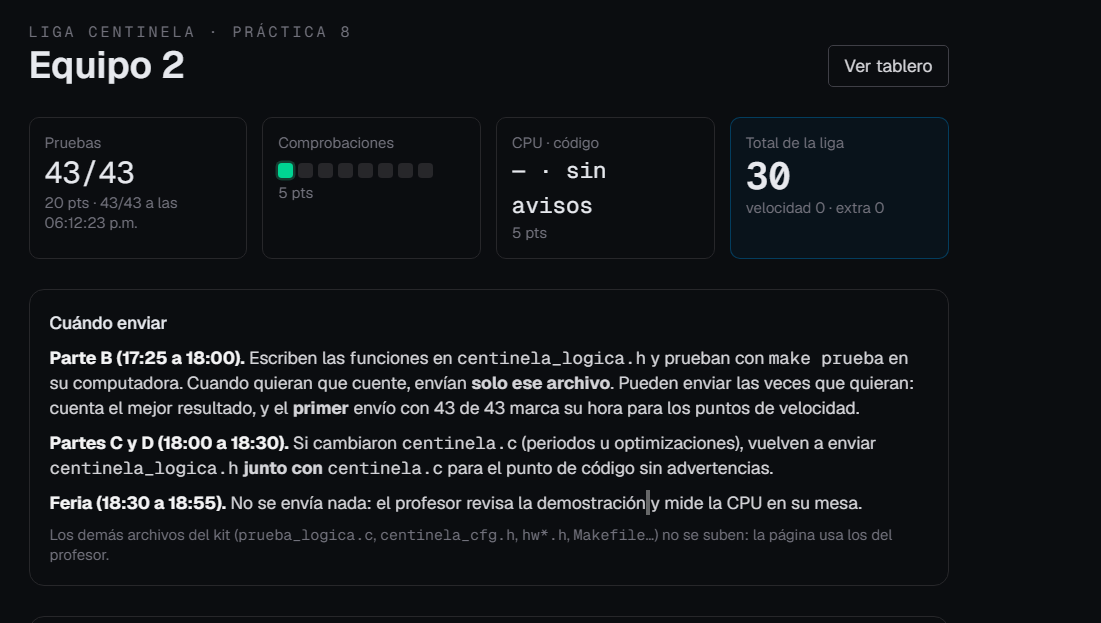
\includegraphics[width=\columnwidth]{C3.png}
    \caption{Tablero de la liga Centinela correspondiente al Equipo 2, con 43 de 43 pruebas y un total mostrado de 30 puntos.}
    \label{fig:c3}
\end{figure}

La Figura~\ref{fig:c3} muestra el resultado de las pruebas de lógica registrado en la plataforma, así como los puntos acumulados al momento de realizar la captura.

\subsection{Parte C. Ejecución del Centinela en el Circuito}

Después de completar la lógica del programa, se procedió a compilar la aplicación para ejecutarla sobre la Raspberry Pi.

Inicialmente se verificó la comunicación I2C mediante el comando \texttt{i2cdetect -y 1}, con la finalidad de identificar la dirección del sensor BMP280.

En la Figura~\ref{fig:c4} se observa que el bus detectó un dispositivo en la dirección \texttt{0x68}, pero no encontró respuesta del BMP280 en la dirección \texttt{0x76}.

\begin{figure}[H]
    \centering
    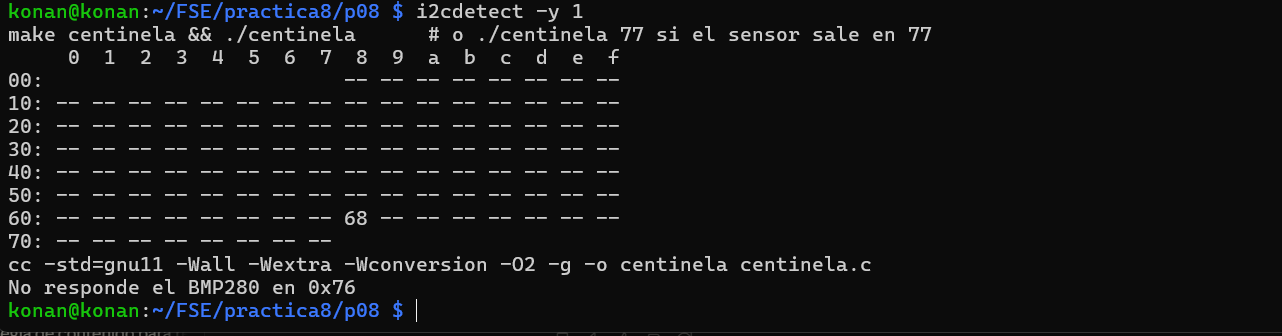
\includegraphics[width=\columnwidth]{C4.png}
    \caption{Exploración del bus I2C y primera ejecución del Centinela, donde se reportó falta de respuesta del BMP280 en la dirección 0x76.}
    \label{fig:c4}
\end{figure}

Este resultado indicó que existía un problema de comunicación con el sensor durante esa comprobación. Por lo tanto, fue necesario revisar la ejecución y continuar con las pruebas del sistema.

En ejecuciones posteriores se observó que Centinela logró calcular una temperatura base y mostrar información sobre los estados, el umbral y el potenciómetro.

\begin{figure}[H]
    \centering
    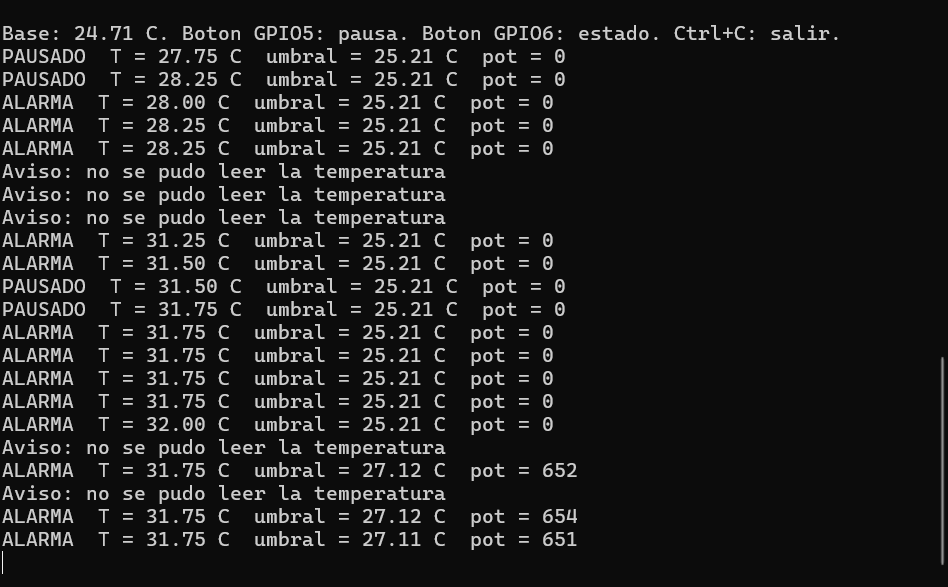
\includegraphics[width=\columnwidth]{C5.png}
    \caption{Ejecución del Centinela con registros de temperatura, umbral y cambios entre los estados PAUSADO y ALARMA.}
    \label{fig:c5}
\end{figure}

Como se aprecia en la Figura~\ref{fig:c5}, el programa inició con una temperatura base de 24.71 grados Celsius y presentó diferentes registros correspondientes a los estados PAUSADO y ALARMA.

También se observó que el valor del potenciómetro modificó el umbral de temperatura. Por ejemplo, con una lectura de 652 se obtuvo un umbral cercano a 27.12 grados Celsius.

Sin embargo, durante la ejecución aparecieron advertencias indicando que algunas lecturas de temperatura no pudieron completarse.

Estas advertencias muestran que la comunicación con el sensor presentó fallas intermitentes, aunque el programa continuó ejecutándose.

Posteriormente, se realizaron más pruebas para observar las transiciones entre estados y la respuesta del sistema ante diferentes temperaturas y posiciones del potenciómetro.

\begin{figure}[H]
    \centering
    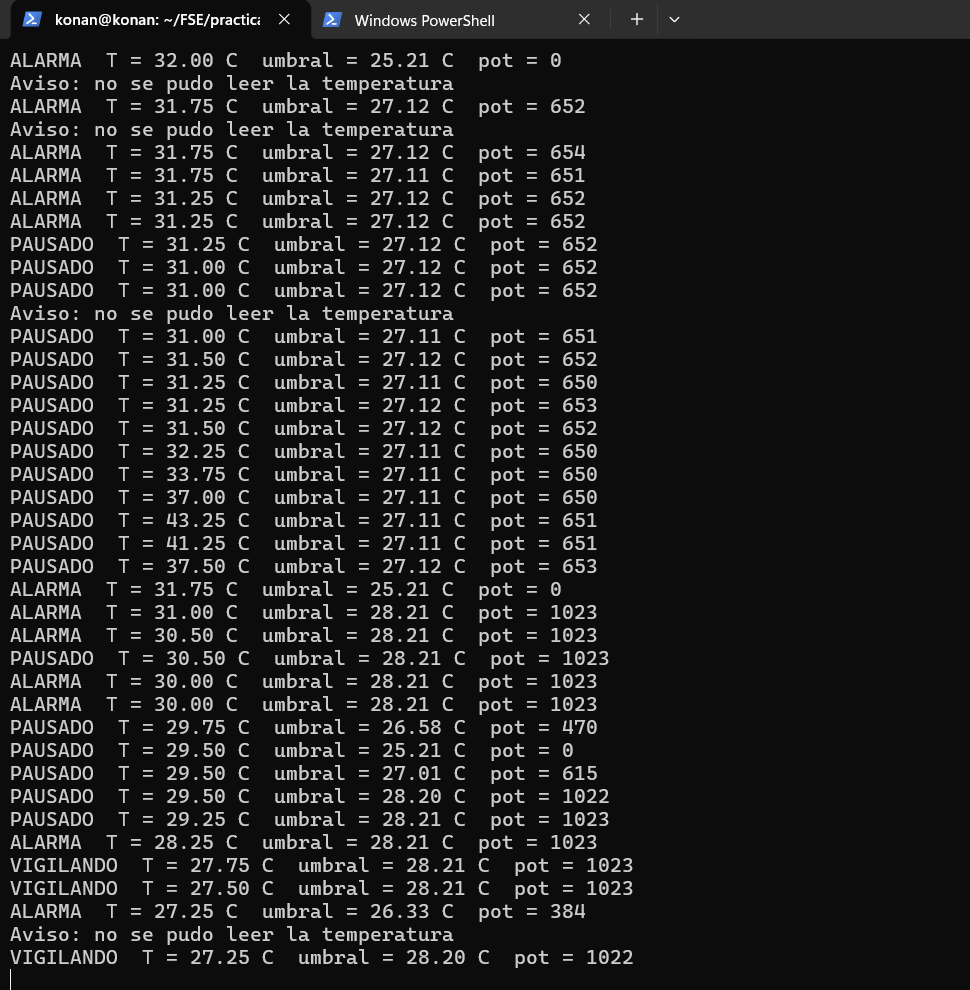
\includegraphics[width=\columnwidth]{C6.png}
    \caption{Comprobación de cambios entre ALARMA, PAUSADO y VIGILANDO, así como variaciones del umbral mediante el potenciómetro.}
    \label{fig:c6}
\end{figure}

En la Figura~\ref{fig:c6} se identifican transiciones entre los tres estados del programa.

También se observa el funcionamiento del umbral ajustable. Al modificar el potenciómetro, el valor de referencia cambió y el programa actualizó su comportamiento dependiendo de la temperatura medida.

Los registros permiten comprobar la ejecución de la máquina de estados, aunque las capturas de terminal no permiten verificar por sí solas todas las condiciones físicas de los LEDs ni el tiempo exacto de respuesta de la alarma.

\subsection{Registro de Mediciones en Archivo CSV}

Como parte de las comprobaciones del sistema, se inspeccionó el archivo \texttt{centinela.csv} utilizando los comandos:

\begin{lstlisting}[language=bash]
head -3 centinela.csv
tail -3 centinela.csv
\end{lstlisting}

Estos comandos permitieron consultar los primeros y últimos registros generados durante la ejecución.

\begin{figure}[H]
    \centering
    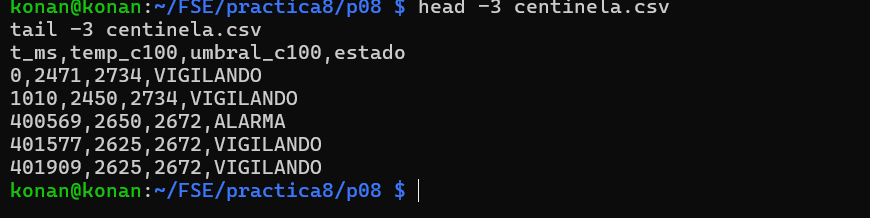
\includegraphics[width=\columnwidth]{C7.png}
    \caption{Inspección del archivo centinela.csv, mostrando el encabezado y registros de temperatura, umbral y estado.}
    \label{fig:c7}
\end{figure}

El archivo presentó la siguiente estructura:

\begin{lstlisting}
t_ms,temp_c100,umbral_c100,estado
0,2471,2734,VIGILANDO
1010,2450,2734,VIGILANDO
400569,2650,2672,ALARMA
401577,2625,2672,VIGILANDO
401909,2625,2672,VIGILANDO
\end{lstlisting}

Los valores de temperatura y umbral se almacenaron en centésimas de grado Celsius.

Por ejemplo, el valor 2471 representa una temperatura de 24.71 grados Celsius, mientras que 2734 corresponde a un umbral de 27.34 grados Celsius.

La diferencia entre los tiempos registrados muestra que el archivo contiene mediciones periódicas y registros asociados con cambios de estado.

Esta información permite analizar posteriormente el comportamiento de la alarma y conservar evidencia de las condiciones registradas durante la ejecución.

\subsection{Parte D. Evaluación de Eficiencia}

La última etapa consistió en evaluar el tiempo de CPU utilizado por Centinela durante intervalos de 60 segundos.

Para ello, se ejecutó el programa en una terminal y, desde otra, se utilizó el script:

\begin{lstlisting}[language=bash]
./medir_cpu.sh 60
\end{lstlisting}

Se realizaron modificaciones a los periodos de lectura de botones y sensores, con la finalidad de comparar diferentes configuraciones.

Las configuraciones identificadas en la evidencia fueron:

\begin{itemize}
    \item Configuración A: botones cada 20 ms y sensor cada 250 ms.
    \item Configuración B: botones cada 1 ms y sensor cada 500 ms.
    \item Configuración final: botones cada 50 ms y sensor cada 500 ms.
\end{itemize}

En la Figura~\ref{fig:c8} se muestran las modificaciones realizadas y las mediciones obtenidas durante las pruebas de eficiencia.

\begin{figure}[H]
    \centering
    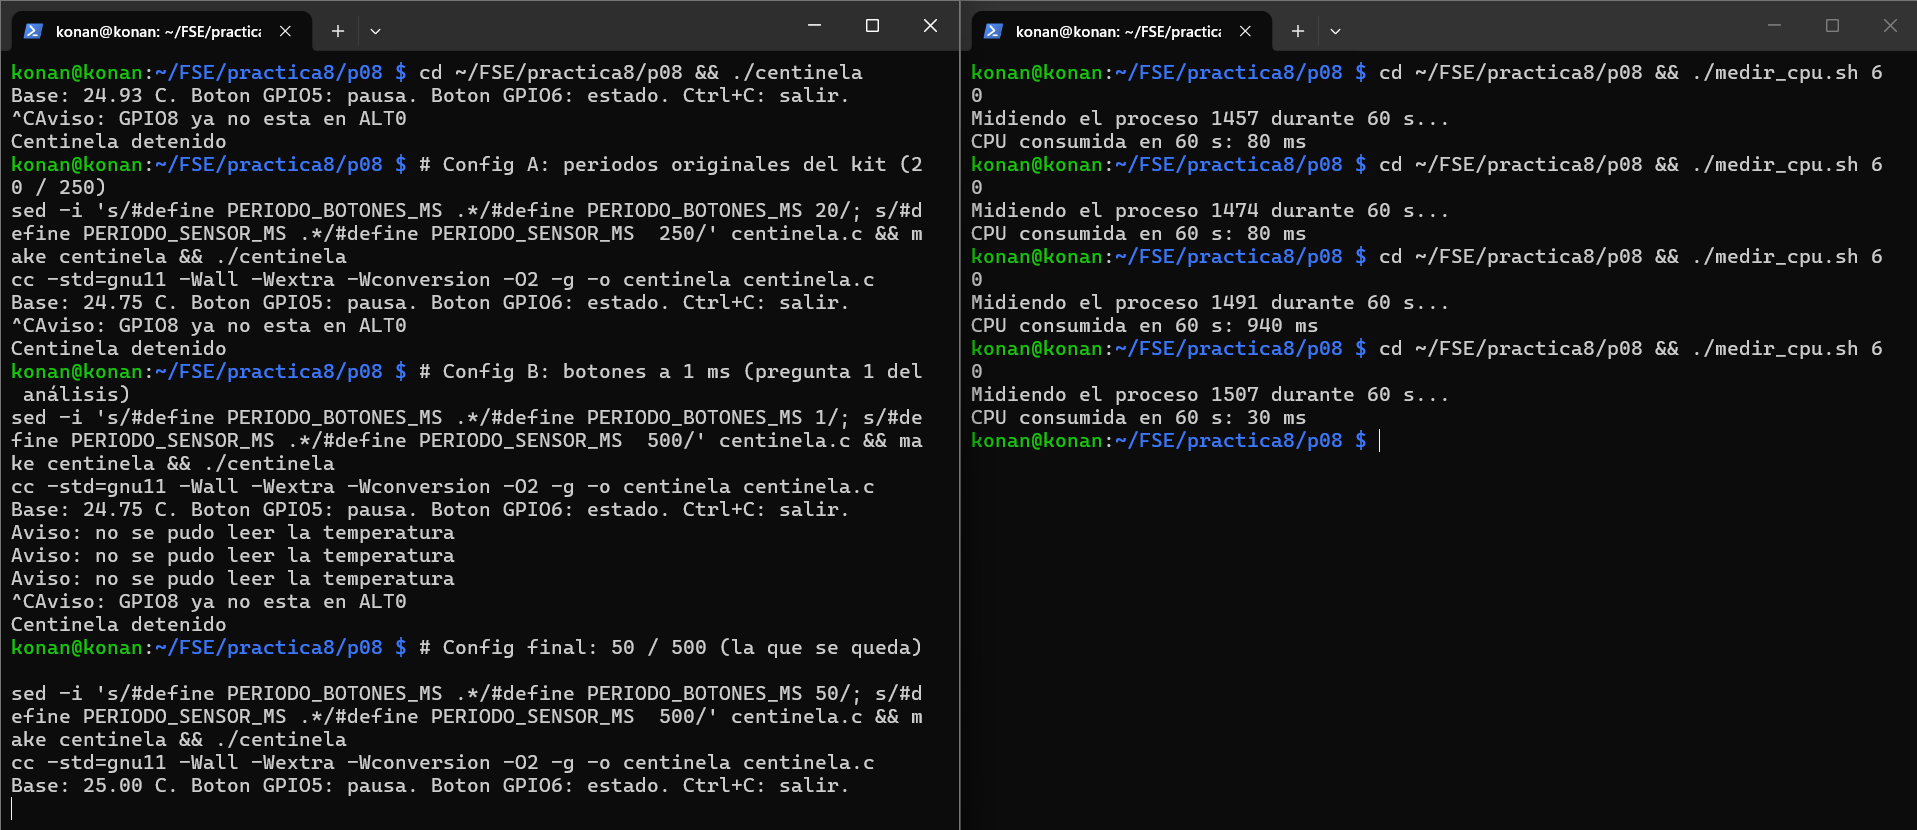
\includegraphics[width=\columnwidth]{C8.png}
    \caption{Modificación de periodos de muestreo y mediciones de tiempo de CPU durante intervalos de 60 segundos.}
    \label{fig:c8}
\end{figure}

Los resultados de CPU registrados fueron de 80, 80, 940 y 30 milisegundos durante intervalos de 60 segundos.

No obstante, la captura no permite asociar con total certeza cada medición a una configuración específica. Por esta razón, los resultados se presentan como mediciones observadas y no como promedios definitivos de cada configuración.

\begin{table}[H]
    \centering
    \caption{Configuraciones utilizadas durante las pruebas de eficiencia}
    \label{tab:configuraciones}
    \scriptsize
    \begin{tabular}{|p{1.65cm}|c|c|}
        \hline
        \textbf{Configuración} &
        \textbf{Botones (ms)} &
        \textbf{Sensor (ms)} \\
        \hline
        A & 20 & 250 \\
        \hline
        B & 1 & 500 \\
        \hline
        Final & 50 & 500 \\
        \hline
    \end{tabular}
\end{table}

\begin{table}[H]
    \centering
    \caption{Mediciones de CPU observadas en la evidencia}
    \label{tab:cpu}
    \scriptsize
    \begin{tabular}{|c|c|}
        \hline
        \textbf{Medición} &
        \textbf{CPU en 60 s (ms)} \\
        \hline
        1 & 80 \\
        \hline
        2 & 80 \\
        \hline
        3 & 940 \\
        \hline
        4 & 30 \\
        \hline
    \end{tabular}
\end{table}

Finalmente, se dejó configurado el programa con un periodo de 50 ms para los botones y 500 ms para el sensor.

Esta decisión buscó disminuir la frecuencia de consulta de los dispositivos y reducir las operaciones realizadas por el procesador, conservando los periodos dentro de los límites permitidos por la práctica.

% =====================================================
% RESULTADOS Y ANÁLISIS
% =====================================================

\section{Resultados y Análisis}

A partir de las pruebas realizadas y de las evidencias presentadas en las Figuras~\ref{fig:c1} a \ref{fig:c8}, se analizaron los resultados obtenidos durante la implementación de Centinela.

\subsection{Validación de la Lógica}

La primera ejecución de las pruebas automáticas obtuvo 7 de 43 casos correctos, debido a que las funciones del kit todavía no estaban implementadas.

Después de completar las funciones correspondientes, se alcanzó un resultado de 43 de 43 pruebas, como se observa en la Figura~\ref{fig:c2}.

Este resultado permitió comprobar que los cálculos del umbral, las máscaras de LEDs, el manejo de estados y el formato de los registros cumplieron con los casos evaluados por las pruebas automáticas.

Asimismo, la plataforma de la liga registró el resultado completo de las pruebas de lógica para el Equipo 2, como se muestra en la Figura~\ref{fig:c3}.

\subsection{Funcionamiento del Sistema en Hardware}

Durante la ejecución se identificaron diferentes comportamientos del programa.

El sistema consiguió calcular una temperatura base, actualizar el umbral a partir del potenciómetro y registrar transiciones entre los estados VIGILANDO, ALARMA y PAUSADO.

Sin embargo, la comunicación con el sensor BMP280 no fue completamente estable.

En la Figura~\ref{fig:c4} se observa que el sensor no respondió en la dirección consultada, mientras que en las Figuras~\ref{fig:c5} y \ref{fig:c6} aparecen advertencias de lectura durante el funcionamiento.

Esto demuestra la importancia de verificar la comunicación con los periféricos, ya que una aplicación puede tener su lógica correctamente implementada y aun así presentar dificultades relacionadas con el hardware.

\subsection{Comprobaciones Funcionales}

La guía de la práctica establece ocho comprobaciones para evaluar el comportamiento de Centinela.

La Tabla~\ref{tab:comprobaciones} resume lo que puede verificarse con las capturas disponibles.

\begin{table}[H]
    \centering
    \caption{Comprobaciones del funcionamiento de Centinela}
    \label{tab:comprobaciones}
    \scriptsize
    \begin{tabular}{|p{2.9cm}|p{3.5cm}|}
        \hline
        \textbf{Comprobación} &
        \textbf{Resultado observado} \\
        \hline
        1. Temperatura base &
        Se observa el cálculo inicial. \\
        \hline
        2. Cambio de umbral &
        Se observan distintos valores del potenciómetro y del umbral. \\
        \hline
        3. Barra de LEDs &
        No verificable directamente con las capturas. \\
        \hline
        4. Activación de alarma &
        Se observa el estado ALARMA, pero no se mide su latencia. \\
        \hline
        5. Histéresis &
        Se observan transiciones; no se documenta una prueba controlada completa. \\
        \hline
        6. Pausa &
        Se observa el estado PAUSADO. \\
        \hline
        7. Archivo CSV &
        Se comprueba la estructura y presencia de registros. \\
        \hline
        8. Salida limpia &
        Se observa el mensaje de detención; la restauración física de pines no queda verificada. \\
        \hline
    \end{tabular}
\end{table}

Las evidencias muestran el funcionamiento de los principales componentes del programa. Sin embargo, para afirmar que se cumplieron las ocho comprobaciones sería necesario contar también con el registro de la evaluación presencial del circuito.

\subsection{Análisis del Registro de Datos}

El archivo \texttt{centinela.csv} permitió comprobar que las mediciones se almacenaron utilizando un formato definido.

Cada línea incluye el tiempo, la temperatura, el umbral y el estado.

El uso de centésimas de grado evita depender de operaciones de punto flotante para representar la temperatura dentro de la lógica principal.

Además, el registro de cambios de estado permite identificar cuándo el sistema entra o sale de la condición de alarma.

\subsection{Análisis del Consumo de CPU}

Las mediciones de CPU mostraron diferencias importantes entre las ejecuciones realizadas.

El menor tiempo observado fue de 30 ms durante una ventana de 60 segundos, mientras que el mayor alcanzó 940 ms.

Esta variación indica que la carga del procesador puede cambiar considerablemente dependiendo de la frecuencia de ejecución y de las condiciones del sistema.

No obstante, debido a que las capturas no identifican inequívocamente la configuración correspondiente a cada medición, no es posible atribuir toda la diferencia únicamente al periodo de lectura de botones.

La configuración final seleccionada fue de 50 ms para botones y 500 ms para sensores, con la intención de reducir la cantidad de consultas realizadas por segundo.

% =====================================================
% PREGUNTAS DE ANÁLISIS
% =====================================================

\subsection{Preguntas de Análisis}

\subsubsection{1. ¿Cómo cambia el tiempo de CPU al establecer PERIODO\_BOTONES\_MS en 1?}

Al reducir el periodo de lectura de botones a 1 ms, el programa necesita revisar las entradas con mayor frecuencia.

Con un periodo de 20 ms se realizan aproximadamente:

\begin{equation}
f = \frac{1000}{20}=50
\end{equation}

consultas por segundo.

En cambio, con un periodo de 1 ms:

\begin{equation}
f = \frac{1000}{1}=1000
\end{equation}

consultas por segundo.

Esto representa 20 veces más consultas de botones respecto a la configuración de 20 ms.

En consecuencia, se espera que aumente el trabajo del procesador asociado con estas lecturas.

Durante la práctica se observaron tiempos de CPU de 80, 80, 940 y 30 ms en diferentes ejecuciones. Sin embargo, no se cuenta con una correspondencia suficientemente clara entre cada resultado y su configuración para calcular un incremento experimental exacto.

Por lo tanto, el efecto esperado es un aumento del consumo de CPU, aunque su magnitud debe comprobarse mediante mediciones controladas con las mismas condiciones de ejecución.

\subsubsection{2. ¿Qué problema causaría eliminar la histéresis cerca del umbral?}

Si se elimina la histéresis, el sistema podría cambiar constantemente entre VIGILANDO y ALARMA cuando la temperatura se encuentre muy cerca del umbral.

Esto ocurriría porque pequeñas variaciones del sensor podrían hacer que una lectura supere el límite y la siguiente quede ligeramente por debajo.

Como consecuencia, los LEDs cambiarían repetidamente de patrón y se generarían más registros de transición.

La histéresis de 0.30 grados Celsius evita este comportamiento al establecer una diferencia entre la temperatura de activación y la de desactivación.

De esta manera, el sistema mantiene un comportamiento más estable frente a pequeñas fluctuaciones de temperatura.

\subsubsection{3. ¿Qué datos podrían perderse si se interrumpe la energía entre sincronizaciones?}

El programa escribe información en el archivo CSV de manera periódica, pero utiliza \texttt{fsync()} principalmente durante los cambios de estado y al finalizar.

Si se interrumpe la alimentación eléctrica durante un periodo sin cambios de estado, algunos registros recientes podrían permanecer únicamente en los búferes del sistema operativo y no haberse almacenado todavía de manera persistente en la microSD.

Por esta razón, podrían perderse las últimas mediciones posteriores a la sincronización más reciente.

La cantidad exacta de información perdida dependería del tiempo transcurrido desde la última sincronización y del comportamiento del sistema de archivos.

Una posible solución sería realizar sincronizaciones periódicas adicionales, aunque esto también aumentaría las operaciones de escritura sobre la microSD.

\subsubsection{4. ¿Qué estado de energía utilizarías entre lecturas para aumentar la duración de la batería?}

Para reducir el consumo de energía utilizaría un mecanismo de espera bloqueante, permitiendo que el proceso permanezca dormido entre las lecturas de sensores y botones.

En Linux, funciones como \texttt{usleep()} permiten suspender temporalmente la ejecución del proceso sin mantener al procesador ocupado consultando continuamente el tiempo.

Esto facilita que el sistema operativo aproveche los periodos de inactividad y utilice estados de reposo de CPU cuando estén disponibles.

En el programa conservaría los periodos de muestreo necesarios, pero evitaría ciclos de espera activa.

También reduciría las lecturas innecesarias del sensor y mantendría apagados los LEDs cuando el sistema se encuentre en PAUSADO.

Es importante mencionar que esta estrategia reduce la actividad del procesador, pero no equivale a suspender completamente la Raspberry Pi. Para conseguir un ahorro mayor sería necesario evaluar las capacidades de administración de energía del hardware.

% =====================================================
% DISCUSIÓN
% =====================================================

\subsection{Discusión General}

El desarrollo de Centinela permitió integrar diferentes conceptos estudiados durante el curso de Fundamentos de Sistemas Embebidos.

Las pruebas automáticas facilitaron la detección de errores en las funciones de cálculo y transición de estados antes de ejecutar el programa sobre el circuito real.

El resultado de 43 de 43 pruebas mostró que la lógica implementada cumplió con los casos de evaluación establecidos.

Por otra parte, las pruebas con el hardware permitieron observar que el funcionamiento de una aplicación embebida no depende únicamente de la corrección del código, sino también de la comunicación con los dispositivos físicos.

Las advertencias relacionadas con el BMP280 evidenciaron que es necesario contemplar fallas de lectura y mantener mecanismos adecuados para manejar errores sin detener inesperadamente el programa.

Finalmente, las mediciones de eficiencia mostraron la importancia de seleccionar correctamente los periodos de muestreo.

Un periodo demasiado corto puede incrementar la carga del procesador, mientras que uno demasiado largo puede retrasar la respuesta del sistema.

Por ello, el diseño debe encontrar un equilibrio entre eficiencia y capacidad de respuesta, considerando las necesidades específicas de la aplicación.

% =====================================================
% CONCLUSIONES INDIVIDUALES
% =====================================================

\section{Conclusiones}

% Cada integrante debe escribir su conclusión personal
% de 5 a 8 líneas, de acuerdo con la guía del profesor.

\textbf{Belmont Muñoz Samuel}.\\
\textit{[Pendiente: agregar conclusión individual de 5 a 8 líneas.]}

\vspace{0.35cm}

\textbf{Domínguez Palacios Jesús Alejandro}.\\
\textit{[Pendiente: agregar conclusión individual de 5 a 8 líneas.]}

\vspace{0.35cm}

\textbf{Dorantes Mejía Emmanuel}.\\
\textit{[Pendiente: agregar conclusión individual de 5 a 8 líneas.]}

\vspace{0.35cm}

\textbf{García Olvera Emiliano}.\\
Con esta práctica pude ver cómo se integran en una sola aplicación la lógica de control, los periféricos y el registro de datos. Pasar de 7 a 43 de 43 pruebas automáticas me mostró lo útil que es validar las funciones de cálculo y transición de estados antes de conectarlas al circuito. La histéresis de 0.30\,$^{\circ}$C resultó clave para que la alarma no cambiara de estado por pequeñas variaciones del sensor cerca del umbral. En hardware, las fallas intermitentes de lectura del BMP280 y la ausencia de respuesta en la dirección 0x76 me recordaron que un programa con lógica correcta también depende de la comunicación con los dispositivos, y que debe manejar errores sin detenerse. Las mediciones de CPU mostraron que los periodos de muestreo influyen en la carga del procesador, aunque para concluir con precisión haría falta repetirlas en condiciones controladas e identificar cada medición con su configuración. Finalmente, entendí que \texttt{fsync()} y el uso de esperas bloqueantes como \texttt{usleep()} son decisiones de diseño que equilibran la confiabilidad de los datos, la eficiencia y la capacidad de respuesta del sistema.

\vspace{0.35cm}

\textbf{Hernández Alonso Antonio Adonahí}.\\
\textit{[Pendiente: agregar conclusión individual de 5 a 8 líneas.]}

\vspace{0.35cm}

\textbf{Jiménez Reyes Alan Yael}.\\
\textit{[Pendiente: agregar conclusión individual de 5 a 8 líneas.]}

% =====================================================
% REFERENCIAS
% =====================================================

\begin{thebibliography}{00}

\bibitem{guia}
K. A. Delgado Vargas,
``Práctica 8. Centinela: Aplicación completa y reto por equipos con el circuito de las prácticas 2 y 3'',
Fundamentos de Sistemas Embebidos,
Facultad de Ingeniería, UNAM, 2026.

\bibitem{kernighan}
B. W. Kernighan y D. M. Ritchie,
\textit{The C Programming Language},
2nd ed. Prentice Hall, 1988.

\bibitem{barr}
M. Barr y A. Massa,
\textit{Programming Embedded Systems},
2nd ed. O'Reilly Media, 2006.

\bibitem{bmp280}
Bosch Sensortec,
``BMP280 Digital Pressure Sensor Datasheet''.
Disponible en:
\url{https://www.bosch-sensortec.com/}

\bibitem{mcp3008}
Microchip Technology,
``MCP3004/MCP3008 Data Sheet''.
Disponible en:
\url{https://www.microchip.com/}

\bibitem{fsync}
Linux man-pages project,
``fsync(2) -- Synchronize a file's in-core state with storage device''.
Disponible en:
\url{https://man7.org/linux/man-pages/man2/fsync.2.html}

\bibitem{usleep}
Linux man-pages project,
``usleep(3) -- Suspend execution for microsecond intervals''.
Disponible en:
\url{https://man7.org/linux/man-pages/man3/usleep.3.html}

\bibitem{proc}
Linux man-pages project,
``proc(5) -- Process information pseudo-filesystem''.
Disponible en:
\url{https://man7.org/linux/man-pages/man5/proc.5.html}

\end{thebibliography}

\end{document}

